\tikzset{
  treenode/.style = {align=center, inner sep=0pt, text centered,
    font=\sffamily},
  arn_t/.style = {treenode, draw=black,
    minimum width=1em, minimum height=1em},
  arn_n/.style = {treenode, circle, white, font=\sffamily\bfseries, draw=black,
    fill=black, text width=1.5em},% arbre rouge noir, noeud noir
  arn_r/.style = {treenode, circle, black, draw=black, 
    text width=1.5em, very thick},% arbre rouge noir, noeud rouge
  arn_x/.style = {treenode, rectangle, draw=black,
    minimum width=1em, minimum height=1em}% arbre rouge noir, nil
}
\usetikzlibrary{arrows}
Generiere den unendlichen Strom der Fibonacci Zahlen.\\
fib(0) = 1\\
fib(1) = 1\\
fib(n) = fib(n-1) + fib(n - 2)\\
1, 1, 2, 3, 5, 8, 13, 21,\ldots\\
\hspace*{20pt} $\uparrow$ ab hier jeweils Summe der beiden Vorgänger\\
\emph{Beobachtung}:\\
\begin{tabular}{ll}
& 1 1 \textcolor{blue} {2}\textcolor{green} {3}\textcolor{red}{5}\\
+& 1 \textcolor{blue}{2} \textcolor{green}{3} \textcolor{red}{5}\\
\hline
&\textcolor{blue}{2} \textcolor{green}{3} \textcolor{red}{5} \textcolor{orange}{8}
\end{tabular}\\
Stream-Diagramm zu fibs:\\
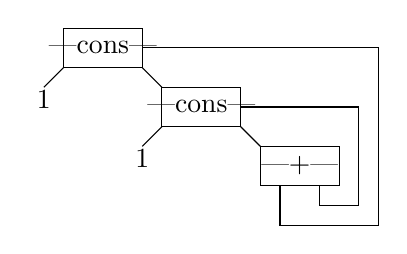
\begin{tikzpicture}
\draw(5,5)rectangle(4,4.5);
\node () at (4.5,4.75) {\lstinline|cons|};
\draw(4,4.5)--(3.75,4.25);
\node () at (3.75,4.10) {1};
\draw(5,4.5)--(5.25,4.25);
\draw(5.25,4.25)rectangle(6.25,3.75);
\node () at (5.75,4) {\lstinline|cons|};
\draw(5.25,3.75)--(5,3.50);
\node () at (5,3.35) {1};
\draw(6.25,3.75)--(6.5,3.5);
\draw(6.5,3.5)rectangle(7.5,3);
\node () at (7,3.25) {\lstinline|+|};
\draw (5,4.75)--(8,4.75)--(8,2.5)--(6.75,2.5)->(6.75,3);
\draw (6.25,4)--(7.75,4)--(7.75,2.75)--(7.25,2.75)--(7.25,3);
\end{tikzpicture}
\rackett{Rekursiv defnierter Sream}{Stream aller Fibonacci Zahlen}{StreamsUndMengen}{201}{225}
\lstinputlisting[firstline=110,lastline=113]{Baeume.rkt}
Die Menge der Binärbäume $T(m)$ ist induktiv definiert:\\
\begin{align}
&\text{\lstinline|empty-tree|} \in T(M) \tag{T1}\\
&\forall x \in M \text{ und } l,r \in T(M): \text{\lstinline|(make-node l x r)|} \in T(M) \tag{T2}\\
&\text{nichts sonst} \t{ in $T(M)$ } \tag{T3}
\end{align}
\emph{Hinweis:}
\begin{enumerate}
\item[-]Jeder Knoten (\lstinline|make-node|) in einem Binärbaum hat zwei Teilbäume sowie eine Markierung (\lstinline|(label)|).
\item[-] Vegleiche:
\subitem $M^*$ und $T(M)$
\subitem \lstinline|empty| und \lstinline|empty-tree|
\subitem \lstinline|make-pair| und \lstinline|make-node|
\end{enumerate}
Visualisierung:
\begin{enumerate}[-]
\item \lstinline|empty-tree| \Box
\item \lstinline|(make-node x l r)|\qquad \begin{minipage}[c]{0.2\textwidth}
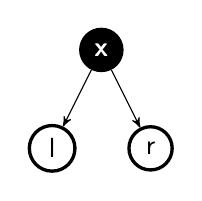
\begin{tikzpicture}[->,>=stealth',level/.style={sibling distance = 1.25cm/#1,
  level distance = 1.25cm}] 
\node [arn_n] {x}
    child{ node [arn_r] {l}                          
    }
    child{ node [arn_r] {r}
		}
; 
\end{tikzpicture}
\end{minipage}
\item Die Knoten mit Markierung x ist \emph{Wurzel} (root) des Baumes
\item Ein Knoten, der nur leere Teilbäume beinhaltet hei\ss t \emph{Blatt} (leaf). Alle anderen Knoten hei\ss en \emph{innere Konten} (inner-nodes)
\end{enumerate}
Beispiel für Binärbäume der Menge $T(M)$\\
\begin{figure}[h!]
\centering
\caption{Baum t}
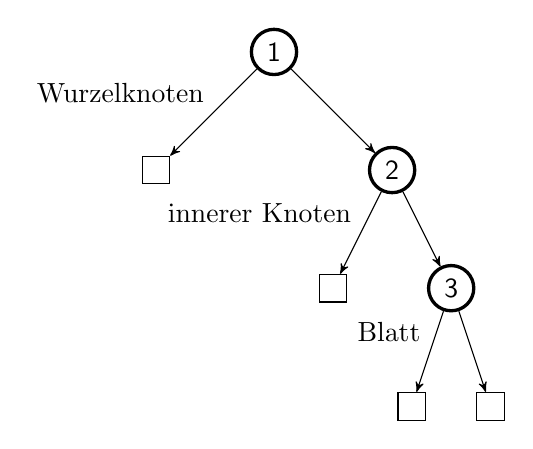
\begin{tikzpicture}[->,>=stealth',level/.style={sibling distance = 3cm/#1,
  level distance = 1.5cm}] 
\node [arn_r] {1}
    child{ node [arn_x] {} edge from parent node[above left]
                         {Wurzelknoten}                            
    }
    child{ node [arn_r] {2}
            child{ node [arn_x] {} edge from parent node[above left]
                         {innerer Knoten}  
            }
            child{ node [arn_r] {3}
							child{ node [arn_x] {} edge from parent node[above left]
                         {Blatt}  }
							child{ node [arn_x] {}}
            }
		}
; 
\end{tikzpicture}
\end{figure}
\begin{figure}[h!]
\centering
\caption{Baum $t_2$ \emph{balanciert}, alle Teilbäume auf einer Tiefe haben die selbe Anzahl an Knoten}
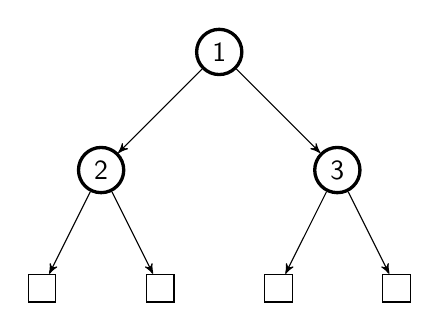
\begin{tikzpicture}[->,>=stealth',level/.style={sibling distance = 3cm/#1,
  level distance = 1.5cm}] 
\node [arn_r] {1}
    child{ node [arn_r] {2}
    child{ node [arn_x] {} 
            }
            child{ node [arn_x] {}}
    }
    child{ node [arn_r] {3}
            child{ node [arn_x] {} 
            }
            child{ node [arn_x] {}}
            }
; 
\end{tikzpicture}
\end{figure}
(Binär-) Bäume haben zahlreiche Anwendungen:
\begin{itemize}
\i Suchbäume (z.B Datenbanken)
\i Datenkompression
\i Darstellung von Termen (Ausdrücken)
\end{itemize}
Bäume sind \emph{die} Induktiv definierte Datenstruktur
\rackett{Implementation von Bäumen}{Verschiedene Bäume}{Baeume}{6}{90}
Die \emph{Tiefe} (depth) eines Baumes ist die maximale Länge eines Weges von der Wurzel von t zu einem leeren Baum.
Also:
\begin{enumerate}[ \ ]
\item \lstinline|(btree-depth empty-tree)| \eval 0
\item \lstinline|(btree-depth t1)| \eval 3
\item \lstinline|(btree-depth t2)| \eval 2
\end{enumerate}
Schablone (gemischte Daten)
\begin{lstlisting}
(: btree-depth ((btree-of %a) -> natural))
(define btree-depth
  (lambda(t)
    (cond ((empty-tree? t) 0)
	  ((node? t) (+ 1
              (max (btree-depth (node-left-branch t))
                   (btree-depth (node-right-branch t))))))
\end{lstlisting}